\chapter{Autonomous Search \& Autotuning}
\label{chap:autonomous}
\epigraph{\textit{There is nothing like looking, if you want to find something. You
certainly usually find something, if you look, but it is not always quite the
something you were after.}}{--- J.R.R. Tolkien, \textit{The Hobbit}}


\section{Algorithm Selection and Autonomous Solvers}
\label{sec:algselres}

In 1976 John R. Rice published \textit{The Algorithm
Problem}~\cite{rice1976algorithm}, an influential paper where he formulated
abstract models for the problem of selecting effective algorithms for a given
problem. In Rice's framework the objective is to select the best algorithm,
according a performance metric, for a given problem. Consider a \textit{problem
space} $P$, and a problem $x \in P$.

Figure~\ref{fig:riceframe} presents Rice's algorithm selection
framework.

\begin{figure}[htpb]
    \begin{center}
        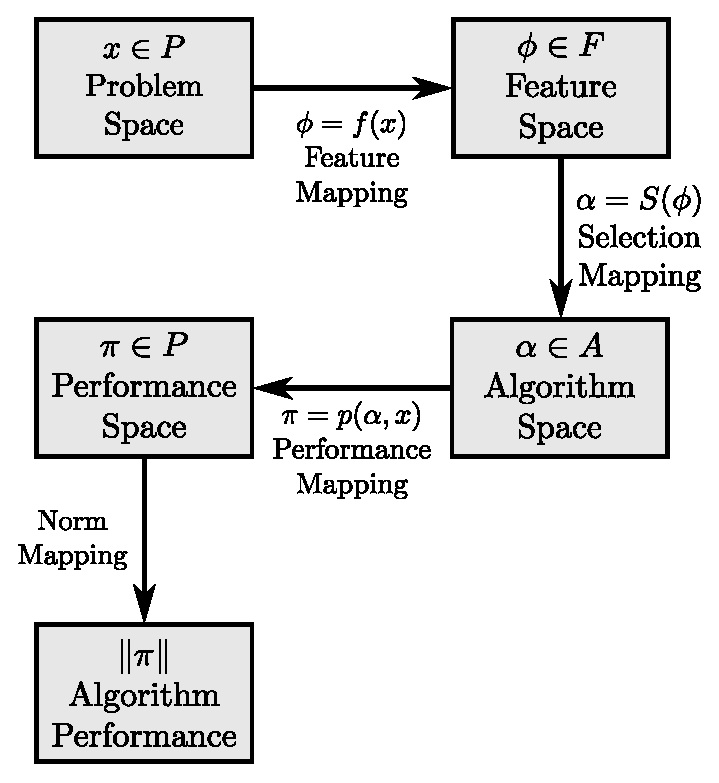
\includegraphics[width=.35\textwidth]{algorithm-selection}
    \end{center}
    \caption{Rice's framework}
    \label{fig:riceframe}
\end{figure}

\todo[inline,author=Pedro,color=cyan]{Discuss autonomous solvers}
\todo[inline,author=Pedro,color=cyan]{Discuss the choice of autotuning for
this work, given all the possibilities for solving the same problem
presented in this chapter}

\section{On-line Control}
\label{sec:oncontrol}

\subsection{Adaptive Parameter Configuration}
\label{subsec:paramadaptive}

\subsection{Credit Assignment}
\label{subsec:creditassign}

\subsection{Reinforcement Learning}
\label{subsec:reinforce}

\section{Off-line Configuration}
\label{sec:offconfig}

\subsection{Evolutionary Computing}
\label{subsec:evolcomp}

\subsection{Stochastic Local Search}
\label{subsec:searchsls}

\subsection{Machine Learning}
\label{subsec:searchml}

\section{Autotuning}
\label{chap:autotuning}

Rice's conceptual framework~\cite{rice1976algorithm} formed the foundation
of autotuners in various problem domains.  In 1997, the PHiPAC
system~\cite{bilmes1997optimizing} used code generators and search scripts to
automatically generate high performance code
for matrix multiplication. Since then, systems tackled different domains with a
diversity of strategies. Whaley \emph{et al.}~\cite{dongarra1998automatically}
introduced the ATLAS project, that optimizes dense matrix multiplication
routines. The OSKI~\cite{vuduc2005oski} library provides automatically tuned
kernels for sparse matrices. The FFTW~\cite{frigo1998fftw} library provides
tuned C subroutines for computing the Discrete Fourier Transform.
Periscope~\cite{gerndt2010automatic} is a distributed online autotuner for
parallel systems and single-node performance.  In an effort to provide a common
representation of multiple parallel programming models, the INSIEME compiler
project~\cite{jordan2012multi} implements abstractions for OpenMP, MPI and
OpenCL, and generates optimized parallel code for heterogeneous multi-core
architectures.

Some systems provide generic tools that enable the implementation of
autotuners in various domains. PetaBricks~\cite{ansel2009petabricks} is a
language, compiler and autotuner that introduces abstractions, such as the
\texttt{\footnotesize either...or} construct, that enable programmers to define
multiple algorithms for the same problem.  The ParamILS
framework~\cite{hutter2009paramils} applies stochastic local search methods
for algorithm configuration and parameter tuning. The OpenTuner
framework~\cite{ansel2014opentuner} provides ensembles of techniques that
search spaces of program configurations. Bosboom \emph{et al.} and Eliahu use
OpenTuner to implement a domain specific language for data-flow
programming~\cite{bosboom2014streamjit} and a framework for recursive parallel
algorithm optimization~\cite{eliahu2015frpa}.

\begin{table}[htpb]
    \centering
    \begin{tabular}{@{}lll@{}}
        \toprule
        System & Domain & Technique \\ \midrule
        ATLAS & Dense Linear Algebra & Exhaustive \\
        INSIEME & Compiler & Genetic Algorithm \\
        SPIRAL & DSP Algorithms & Pareto Active Learning \\
        Active Harmony & Runtime & Nelder-Mead \\
        Periscope & HPC Applications & Various \\
        OpenTuner & Domain-Agnostic & Ensemble \\ \bottomrule
    \end{tabular}
    \caption{Some autotuning systems, their domains and techniques}
\end{table}

Petabricks~\cite{ansel2009petabricks} is a language and compiler that enables
the expression of program implementation search spaces at language level.
OpenTuner~\cite{ansel2014opentuner} is a domain-agnostic autotuning framework
that provides ensembles of search techniques for user-defined program
configurations.

Williams~\cite{williams2009optimization} present optimization strategies for
the sparse matrix-vector multiply kernel in multi-core processors.  Williams et
al.~\cite{williams2009roofline} also present Roofline, a visual performance
model for parallel hardware and software that helps in the optimization of
floating-point computations.

Tartara and Reghizzi~\cite{tartara2012parallel} use the MapReduce programming
model to improve the performance of machine learning algorithms in the
PetaBricks compiler. Later they presented a machine learning
algorithm~\cite{tartara2013continuous} that learns compiler heuristics using
data gathered after every compilation.

LGen~\cite{spampinato2014basic} is a compiler for small-scale linear algebra
computation that uses mathematical domain-specific languages to optimize loops
and vectorization. LGen uses exhaustive or random search to test different
optimizations.

TuningGenie~\cite{ivanenko2014method} presents an autotuning framework that
uses code annotations for generating autotuners for parallel programs.

Hou et al.~\cite{hou2017auto} present an autotuning framework that uses
decision trees to optimize the sparse matrix-vector multiply kernel
for multi and many-core processors.

Takizawa et al.~\cite{takizawa2017customizable} use OpenTuner and
Xevolver~\cite{takizawa2014xevolver}, a code transformation framework, to
enable the autotuning of code transformations in applications that were not
implemented for autotuning. They present an autotuning ``scenario template''
that uses compiler directives to inform the autotuner.

Panda~\cite{sourouri2017panda} is compiler framework that uses code annotations
to optimize 3D Stencil computations on heterogeneous architectures with CPUs
and GPUs.

Lang~\cite{lang2017data} reviews work on autotuning based on analytical
performance models, arguing that the approach is feasible.

Apollo~\cite{beckingsale2017apollo} is an autotuning framework for
input-dependent kernels that uses a decision tree classifier that provides
optimizations that can be selected during runtime.

Shuchart et al.~\cite{schuchart2017readex} introduce the READEX (Runtime
Exploitation of Application Dynamism for Energy-efficient eXascale computing)
project and its methodology for developing tools to improve the energy
efficiency of High-Performance Computing applications.

Falsch and Elster~\cite{falch2017machine} build performance models for
OpenCL applications in different target architectures using machine learning.
A statistical model learned and later used to pick promising configurations for
testing.

The Periscope Tuning Framework
(PTF)~\cite{gerndt2005periscope,gerndt2010automatic,gerndt2017multi} is an
online tool for performance analysis and tuning that has a modular architecture
based on plugins.

Xu et al.~\cite{xu2017parallel} present an autotuning strategy that uses
parallel OpenTuner instances to autotune the FPGA compilation flow.  Their work
dynamically partition the search space between MPI-communicating OpenTuner
instances.

Abdelfattah et al.~\cite{abdelfattah2016performance} present an autotuning
strategy using exhaustive evaluation of General Matrix-Matrix Multiply (GEMM)
kernel optimizations for GPUs. They later use this approach to optimize GPU
kernels for large-scale tensor contractions~\cite{abdelfattah2016high}.

Active Harmony~\cite{tapus2002active} provides an API that enables
online autotuning of a program using a variation of the Nelder-Mead
simplex algorithm~\cite{nelder1965simplex}.

MASE-BDI~\cite{coelho2016mase} is a multi-agent system for the simulation of
environmental land change that uses the Active Harmony
API~\cite{tapus2002active} and search algorithms to autotune its parameters.
Several simulator configurations are executed in parallel and communicate their
results to a tuning manager using MPI.

Xu et al.~\cite{xu2016analytical} introduce an autotuning framework for
loop scheduling in GPUs that uses analytical performance models.

TANGRAM~\cite{chang2015tangram,chang2016efficient} is a kernel
synthesis framework for different architecture hierarchies.
It uses composition rules and breadth-first search to prune
and explore the design space.

Balaprakash et al.~\cite{balaprakash2016automomml} introduce a framework
that uses machine learning algorithms to build models for metrics such as
performance and energy consumption, which are used for multi-objective
optimization.

Ngoko et al.~\cite{ngoko2016automatic} introduce an autotuning system for
$\NP$-hard problems that uses distributed measurements of configurations and
machine learning algorithms aided by randomization, clustering and set
intersection solvers.

Ziegler et al.~\cite{ziegler2016synthesis,ziegler2016scalable} present an
autotuning system for hardware synthesis parameters that uses genetic and
learning algorithms to explore the hardware design space for real industrial
chip designs from IBM.

Jayasena et al.~\cite{jayasena2015auto} use OpenTuner to implement an autotuner
for a Java Virtual Machine implementation.

Luo et al.~\cite{luo2015fast} present a framework for stencil computations that
uses Optimal-Solution Spaces, input feature extraction and machine learning.

Guerreiro et al.~\cite{guerreiro2015multi} use search space pruning strategies
and exhaustive evaluation to autotune CUDA GPU kernels.

Garvey et al.~\cite{garvey2015automatic} present a strategy to autotune OpenCL
GPU kernels using machine learning, heuristics for search space partitioning
and exhaustive search.

CLTune~\cite{nugteren2015cltune} is an autotuning framework for OpenCL kernels
that uses search algorithms such as simulated annealing and particle swarm
optimization.

Mametjanov et al.~\cite{mametjanov2015autotuning} present an autotuning
approach that uses machine learning and selective sampling of the search space
to optimize FPGA hardware design parameters for performance and power.

PolyMage~\cite{mullapudi2015polymage} is a domain-specific language and
compiler for image processing pipelines. It uses heuristics and performance
models to prune the search space, which is then explored exhaustively.

\subsection{OpenTuner}
\label{sec:opentuner}
\todo[inline,author=Pedro,color=cyan]{Discuss OpenTuner's limitations and shortcomings.}

\subsubsection{Context}
\label{sec:context}

\subsubsection{Software Architecture}
\label{sec:arch}

\subsubsection{Parallel and Distributed Programming in OpenTuner}
\label{sec:opentuner-parallel}
\todo[inline,author=Pedro,color=cyan]{Discuss the difficulties and
explain why they motivated the new Julia code.}

\subsection{Search Techniques}
\label{sec:techniques}

\subsubsection{Numerical Methods}
\label{subsec:num}

\subsubsection{Evolutionary Computation}
\label{subsec:tuninevolcomp}

\subsubsection{Stochastic Local Search}
\label{subsec:tuningsls}

\subsubsection{Machine Learning}
\label{subsec:tuningml}

\subsection{Benchmarks}
\label{sec:benchmarks}

\subsubsection{Solvers of NP-Complete Problems}
\label{subsec:np}

\subsubsection{Algorithm Selection and Configuration}
\label{subsec:algsel}

\subsubsection{Compiler Configuration}
\label{subsec:compilerconfig}

\subsubsection{Measurement Time}
\label{subsec:measure}
